\chapter{Solución de ecuaciones lineales de dimensiones no pequeñas}\label{chapter:solve-non-smal-lineal-eq}

En el capítulo anterior, se presentó la discretización Lineal Local~(\ref{ODE-LLA-4}) de EDO, así como su implementación basada en aproximantes de Padé~(\ref{LL-scheme}) para pequeños PVI. Sin embargo, para PVI de medianas y grandes dimensiones, la aproximación de Padé~(\ref{P-MA-2}) no es computacionalmente eficiente y necesita ser reemplazada por otra aproximación basada en subespacios de Krylov o alguna técnica proyectiva similar. Nótese que, para la ecuación lineal
\begin{equation*}
	\frac{dx(t)}{dt}=Ax(t)\;,\;\; x(t_0)=x_0,\;\;\; A\in\mathbb{R}^{d\times d}\;,
\end{equation*}
además de la solución en forma integral, la solución también puede ser escrita de las siguientes formas
\begin{eqnarray}
	x(t) & = & \me{tA}x_0 \label{eqaux:lineal-solution-ex} \\
	x(t) & = & x_0 + L\me{tM}r \label{eqaux:lineal-solution-xex} \\
	x(t) & = & x_0 + t\varphi_1(tA)Ax_0 \label{eqaux:lineal-solution-xphix}
\end{eqnarray}
donde $\varphi_1$ está definida en (\ref{phi-definition}) y
\begin{equation*}
	L=\left[ \begin{array}{ll} I_{d} & 0_{d\times 1}\end{array} \right] \;,\;\;
	r^{\intercal }=\left[ \begin{array}{ll} \mathbf{0}_{1\times d} & 1\end{array}\right] \;,\;\;
	M=\left[
	\begin{array}{cc}
	A & Ax_0 \\
	0 & 0
	\end{array}
	\right]\;.
\end{equation*}
Cada una de estas formas de la solución puede ser aproximaciones utilizando subespacios Krylov. En los trabajos~\cite{Saad92,jimenez2012convergence} se utilizan aproximaciones de Krylov para las soluciones de las forma~(\ref{eqaux:lineal-solution-ex},\ref{eqaux:lineal-solution-xex}). Dichas aproximaciones son de orden $\mf$, donde $\mf$ es la dimensión del subespacio utilizado. En cambio para la solución de la forma~(\ref{eqaux:lineal-solution-xphix}) se han utilizado aproximaciones de orden  $\mf+1$~\cite{sidje1998expokit,niesen2012algorithm}. En este capítulo se introducirán aproximaciones Krylov-Padé de un orden mayor para la acción de $\varphi_1$, así como una variante que no evalúa la matriz Jacobiana. También se derivarán cotas para las aproximaciones propuestas y se propondrá una estrategia para la selección de la dimensión de los subespacios de Krylov. Los resultados de este capítulo están basados en \cite{naranjo2023computing,naranjo2023RT,naranjo2021locally,naranjo2023jacobian}.

\section{Aproximaciones Krylov-Padé a la acción del operador phi}\label{section:krylov-pade-approx}

Como se explicó en el Capítulo anterior, la acción del operador $\varphi_1$ definida como el producto de la función $\varphi_1$ por vector tiene un papel fundamental en las discretizaciones Lineales Locales de la solución de (\ref{ODE-SYST}) por lo que se hace indispensable evaluar dicha operación de forma rápida y precisa. Con ese propósito, el truncamiento de la serie~(\ref{PHI-EXPANSION}) es útil. Típicamente~\cite{niesen2012algorithm,sidje1998expokit,tokman2006efficient}, el primer término de la serie es tomado como aproximación y el segundo término es utilizado como medida del error; pero, en este trabajo, similar a~\cite{Saad92} se tomarán los dos primeros términos de la serie (\ref{PHI-EXPANSION})
 \begin{equation}\label{exact-two-terms-km}
    K_\mf(\tau,A,b) = \norme{b}\tau V_\mf\varphi_1(\tau H_\mf)e_1 + \norme{b}\tau^2\hf_{\mf+1,\mf}e^T_\mf\varphi_2(\tau H_\mf)e_1v_{\mf+1}
 \end{equation}
para aproximar $\tau\varphi_1(\tau A)b$ y el tercer término como medida del error.

Al aplicar conjuntamente el Algoritmo de Arnoldi \ref{alg:Arnoldi}, la propiedad de invarianza ante escalado de la base ortonormal del subespacio de Krylov y el Teorema \ref{theorem:exp-phi} podemos evaluar la acción de las $\varphi_j$ en (\ref{exact-two-terms-km}) calculado una exponencial matricial. En efecto, con la matriz de Hessenberg $H^*_\mf$ resultante de aplicar el Algoritmo \ref{alg:Arnoldi} para $\mathcal{K}_\mf(\tau A,b)$ se obtiene la matriz de Hessenberg $H_\mf=H^*_\mf/\tau$ correspondiente a $\mathcal{K}_\mf(A,b)$ y, de ésta forma, se puede calcular la exponencial de la matriz particionada
\begin{equation}
    \overline{H} = \left[\begin{array}{cccc}
    H_\mf & e_1 & 0_{\mf\times 1} & 0_{\mf\times 1}\\
    0_{1\times\mf} & 0 & 1 & 0\\
    0_{1\times\mf} & 0 & 0 & 1\\
    0_{1\times\mf} & 0 & 0 & 0
    \end{array}\right] \label{hhat_hessenberg_matrix}
    \end{equation}
para obtener la identidad
\begin{equation}
    \me{\tau\overline{H}} = \left[\begin{array}{cccc}
    \me{\tau H_m} & \tau\varphi_1(\tau H_m)e_1 & \tau^{2}\varphi_2(\tau H_m)e_1 &
    \tau^{3}\varphi_3(\tau H_m)e_1 \\
    & 1 & \tau & \frac{\tau^{2}}{2}\\
    &  & 1 & \tau \\
    &   &   & 1 \\
    \end{array}\right] \,. \label{phi_hhat_exponential}
\end{equation}
del Teorema \ref{theorem:exp-phi}.

Al aplicar (\ref{phi_hhat_exponential}) en (\ref{exact-two-terms-km}) se obtiene
\begin{equation*}
    K_\mf(\tau,A,b) = \norme{b}V_\mf [E_\tau]_{12} + \norme{b}\hf_{\mf+1,\mf}e^T_\mf[E_\tau]_{13}v_{\mf+1}, 
 \end{equation*}
 donde $E_\tau = \me{\tau \overline{H} }$ y $[E_\tau]_{ij}$ denota las particiones de la matriz $E_\tau$. Como, en general, la exponencial matricial $E_\tau$ no se puede calcular de forma exacta, se utiliza la aproximación
\begin{equation*}
    \widetilde{E}_{\tau} = F_k^{\pf,\qf}\left(\tau\overline{H}\right),
\end{equation*}
donde $F_k^{\pf,\qf}$ denota la aproximación de Padé-($\pf,\qf$) con escalamiento y potenciación $k$ definida en~(\ref{P-MA-2}). Con ésta nueva aproximación, se obtiene la expresión 
\begin{equation} \label{eq:kp_aprox}
    K_{\mf,k}^{\pf,\qf}(\tau,A,b) = \norme{b}V_\mf [\widetilde{E}_\tau]_{12} + \norme{b}\hf_{\mf+1,\mf}e^T_\mf[\widetilde{E}_\tau]_{13}v_{\mf+1}
 \end{equation}
 que define a la aproximación de Krylov-Padé para $\tau\varphi_1(\tau A)b$.

 \subsection{Cotas para las aproximaciones}
 En está sección se enunciará un teorema para acotar el error de la aproximación (\ref{eq:kp_aprox}) en función de $\tau$, la dimensión del subespacio de Krylov $\mf$ y los órdenes de Padé $\pf$ y $\qf$. Para poder enunciar dicho teorema dos lemas adicionales son necesarios. El primer lema extiende para $\tau \varphi_1(\tau A)b$ los resultados del Teorema 4.7 en~\cite{Saad92} para aproximaciones de $\varphi_0(A)b$ mediante subespacios de Krylov. El segundo lema ofrece una cota para la matriz $\overline{H}$.

 \begin{lemma}\cite{naranjo2021locally}\label{lemma:CORRECTED-ERROR}
	Sea $A\in\mathbb{C}^{d\times d}$ una matriz, $b\in\mathbb{C}^{d}$ un vector, $\tau$ un número positivo, y \[{K_{\mf}\left(\tau,A , b \right) = \tau ||b||_2 V_\mf \varphi_1(\tau H_\mf)e_1}+\tau^2 ||b||_2 \hf_{\mf+1,\mf}e_\mf^T\varphi_2\left(\tau H_\mf\right) e_1 v_{\mf+1} \] la aproximación a $\tau \varphi_1(\tau A)b$ tomando los dos primeros términos de la serie (\ref{PHI-EXPANSION}). Entonces,
	\begin{gather*}
	\left\lvert\left\lvert \tau\varphi_1(\tau A)b - K_{\mf}\left(\tau,A , b \right) \right\rvert\right\rvert_2%\nonumber\\
	\leq \frac{2\vert\lvert b \rvert\rvert_2\tau^{\mf+2}\rho^{\mf+1}\me{\tau \rho}}{(\mf+2)!},
	\end{gather*}
	donde $\rho=\nnorm{\nnorm{A}}_2$.
\end{lemma}
\textbf{Demostración}
Siguiendo la definición (\ref{phi-definition}), $\tau \varphi_1(\tau A)b$ puede ser reescrito como
\begin{eqnarray*}
	\tau \varphi_1(\tau A)b &=& \tau b+\tau^{2}A\varphi_{2}(\tau A)b \\
	&=& \tau b+\tau^{2}A \,\ (\,\ \nnorm{\nnorm{b}}_2V_\mf\varphi_{2}(\tau H_\mf)e_1 +s_\mf(\tau A) \,\ ), %\label{eq:tauaphi1tauab}
\end{eqnarray*}
donde \[ s_\mf (\tau A)= \varphi_{2}(\tau A)b -\nnorm{\nnorm{b}}_2V_\mf\varphi_{2}(\tau H_\mf)e_1 .\]
Utilizando la rescritura de $\varphi_1$, y las identidades $AV_\mf=V_\mf H_\mf + \hf_{\mf+1,\mf}v_{\mf+1}e^{T}_\mf$ y  $\nnorm{\nnorm{b}}_2V_\mf e_1=b$ se obtiene
\begin{equation}
\tau\varphi_1(\tau A)b = \tau\nnorm{\nnorm{b}}_2V_\mf\varphi_1(\tau H_\mf)e_1 + \tau^{2}\nnorm{\nnorm{b}}_2\hf_{\mf+1,\mf}e^T_\mf\varphi_{2}(\tau H_\mf)e_1v_{\mf+1}+\tau^{2}As_\mf (\tau A), %\label{eq:tauaphi1tauabapprox}
\end{equation}
y se tiene que
\begin{equation}
\tau\varphi_1(\tau A)b - K_{\mf}\left(\tau,A , b \right) = \tau^{2}As_\mf(\tau A), \label{eq:phidiffasm}
\end{equation}
donde \[{K_{\mf}\left(\tau,A , b \right) = \tau ||b||_2 V_\mf \varphi_1(\tau H_\mf)e_1}+\tau^2 ||b||_2 \hf_{\mf+1,\mf}e_\mf^T\varphi_2\left(\tau H_\mf\right) e_1 v_{\mf+1} \] es una aproximación de $\tau \varphi_1(\tau A)b$.

Utilizando el Lema 4.1 en \cite{Saad92} se tiene
\begin{equation}
s_\mf(\tau A)=\nnorm{\nnorm{b}}_2 ( r_\mf(\tau A)v_1-V_\mf r_\mf(\tau H_\mf)e_1) ,\label{eq:smeq}
\end{equation}
donde $r_\mf(z) = \varphi_{2}(z)-p_{2,\mf-1}(z)$, y $p_{2,\mf-1}$ es un polinomio de grado $\mf-1$. Tomando
\begin{equation*}
p_{2,\mf-1}(z)\equiv \frac{p_{1,\mf}(z)-1}{z},
\end{equation*}
donde $p_{1,\mf}$ es la expansión de Taylor de $\varphi_1$ hasta el orden  $\mf$
definida por
\[ p_{1,\mf}(z)= \frac{p_{0,\mf+1}(z)-1}{z}, \]
donde $p_{0,\mf+1}(z)$  es la expansión de Taylor de $\me{z}$ hasta el orden $\mf+1$ dada por
\[ p_{0,m+1}(z)=\sum\limits^{\mf+1}_{j=0}\frac{z^j}{j!}. \]

Con estos polinomios y (\ref{phi-definition}) se tiene
\begin{equation*}
r_\mf(z) = \frac{\varphi_1(z)-1}{z}-\frac{p_{1,\mf}(z)-1}{z}=\frac{\me{z}-1}{z^2}-\frac{p_{0,m+1}(z)-1}{z^2}
=\frac{\me{z}-p_{0,m+1}(z)}{z^2}.
\end{equation*}

El Lema 4.2 en \cite{Saad92} enuncia que
\[ \nnorm{\me{z}-p_{0,m+1}(z)} \leq \frac{z^{\mf+2}\me{z}}{(\mf+2)!}\;\;, \]
de esto se obtiene
\begin{equation}
\nnorm{\nnorm{r_\mf(\tau A)v_1}}_2\leq \frac{\rho^{\mf}\me{\rho}}{(\mf+2)!}\;\;\;\;\; y \;\;\;\;\; \nnorm{\nnorm{r_\mf(\tau H_\mf)v_1}}_2\leq \frac{\widehat{\rho}^{\mf}\me{\widehat{\rho}}}{(\mf+2)!}, \label{polinom}
\end{equation}
donde $\rho=\nnorm{\nnorm{\tau A}}_2 $ y  $\widehat{\rho}=\nnorm{\nnorm{\tau H_\mf}}_2$. Ya que $\nnorm{\nnorm{H_\mf}}_2\leq\nnorm{\nnorm{A}}_2$, de (\ref{eq:smeq}) y (\ref{polinom}) se obtiene
\begin{equation*}
\nnorm{\nnorm{\tau As_\mf(\tau A)}}_2  \leq \frac{2 \nnorm{\nnorm{b}}_2\rho^{\mf+1}\me{\rho}}{(\mf+2)!}.
\end{equation*}
Finalmente, de estas desigualdades y (\ref{eq:phidiffasm}) se obtiene
\begin{equation*}
\nnorm{\nnorm{\tau\varphi_1(\tau A)b - K_{\mf}\left(\tau,A , b \right)}}_2  \leq
\frac{2 \nnorm{\nnorm{b}}_2\tau^{\mf+2}\nnorm{\nnorm{A}}_2^{\mf+1}\me{\tau \nnorm{\nnorm{A}}_2}}{(\mf+2)!},
\end{equation*}
lo cual completa la prueba. $\Box$

\begin{lemma}\cite{naranjo2021locally}\label{H-bound}
	Sea $\overline{H}$ la matriz definida en~(\ref{hhat_hessenberg_matrix}), sea  $H_\mf=V^{T}_\mf AV_\mf$ la matriz de Hessenberg asociada al subespacio de Krylov $\mathcal{K}_\mf(A,b)$ con base ortonormal $V_m$. Entonces
	\[ \lVert\overline{H}\rVert_2 \leq 1 +  \lVert A\rVert_2. \]
\end{lemma}
\emph{Demostración}
De (\ref{hhat_hessenberg_matrix}) se tiene
\begin{eqnarray*}
	\overline{H}&=&L H_\mf L^T + B
\end{eqnarray*}
donde $ L^T=[I_\mf \;\; 0_{\mf\times 3}] $ y
\[B=\left[\begin{array}{ccc}
0_{\mf\times\mf} & e_1 & 0_{\mf \times 2}\\
0_{2\times\mf} & 0_{2 \times 1} & I_2\\
0_{1\times\mf} & 0 & 0_{1\times 2}
\end{array}\right].\]
Ya que $\lVert B\rVert_2 = \lVert L \rVert_2 = 1$, y $\lVert H_m\rVert_2 \le \lVert A \rVert_2$, se obtiene que
\begin{eqnarray*}
	\lVert\overline{H}\rVert_2 &\leq& \lVert L \rVert_2 \lVert H_\mf \rVert_2 \lVert L^T \rVert_2 + \lVert B \rVert_2\\
	&\leq& 1 + \lVert A\rVert_2
\end{eqnarray*}
$\Box$\\ \\


\begin{theorem}\cite{naranjo2021locally}\label{theorem:Krylov-bound}
	Sea
	\begin{equation} \label{eq:gen_kp_aprox}
	K_{\mf,k}^{\pf,\qf}\left(\tau, A , b \right)=\nnorm{\nnorm{b}}_2 V_{\mf}\;[\widetilde{E}_{\tau}]_{12} + \nnorm{\nnorm{b}}_2 \hf_{\mf+1,\mf}e_\mf^T\;[\widetilde{E}_{\tau}]_{13} v_{\mf+1}
	\end{equation}
	la aproximación $(\mf , \pf ,\qf , k)$-Krylov-Padé de $\tau \varphi_1(\tau A)b$, donde las matrices $V_{\mf}\in\mathbb{R}^{d\times \mf}$ y $H_{\mf}\in\mathbb{R}^{{\mf} \times {\mf}}$, el vector $v_{\mf+1}$, y el número $\hf_{\mf+1,\mf}$ son obtenidos del Algoritmo de Arnoldi para el $\mf$-ésimo subespacio de Krylov $\mathcal{K}_\mf(A,b)$;  $\widetilde{E}_{\tau}=F_k^{\pf,\qf}\left(\tau\overline{H}\right)$ es la aproximación $(\pf,\qf)$-Padé con escalamiento $k$ para la exponencial matricial (\ref{phi_hhat_exponential}), y $e_m$ el $m$-ésimo vector canónico de $\mathbb{R}^\mf$.
	Entonces,
	\begin{equation}
	\left\lvert\left\lvert  \tau \varphi_1(\tau A)b -
	K_{\mf,k}^{\pf,\qf}\left( \tau, A , b \right)\right\rvert\right\rvert_2%\nonumber\\
	\leq C_{\mf,k}^{\pf,\qf}\left(\lvert\lvert A \rvert\rvert_2\right) \;
	\nnorm{\nnorm{b}}_2 \; \tau^{\mathrm{min}\left\{ \mf+2,\pf+\qf+1 \right\}}
	\end{equation}
	donde $C_{\mf,k}^{\pf,\qf}(\varLambda)= \frac{2 \varLambda^{m+1} \me{\varLambda}}{(\mf+2)!}+
	\alpha (1+\hf_{\mf+1,\mf}) (1+\varLambda^{p+q+1}) 2^{-k(\pf+\qf)+3}\me{(1+\alpha(\frac{1}{2})^{\pf+\qf-3})(1+\varLambda)} $,
	con $\alpha=\frac{\pf!\qf!}{(\pf+\qf)!(\pf+\qf+1)!}$ y $\tau \in [0,1]$.
\end{theorem}
\textbf{Demostración} Por desigualdad triangular
\begin{eqnarray} \label{importatdeq}
\left\lvert\left\lvert  \tau \varphi_1(\tau A)b -
K_{\mf,k}^{\pf,\qf}\left( \tau , A , b \right)\right\rvert\right\rvert_2
& \leq & \left\lvert\left\lvert \tau \phi_1(\tau A)b -  K_{\mf}\left( \tau , A , b \right) \right\rvert\right\rvert_2 \\
& & + \left\lvert\left\lvert  K_{\mf}\left( \tau , A , b \right) -
K_{\mf,k}^{\pf,\qf}\left( \tau, A , b \right)\right\rvert\right\rvert_2, \nonumber
\end{eqnarray}
donde
\begin{equation*}
K_{\mf}\left(\tau,A , b \right)=\nnorm{\nnorm{b}}_2 \tau V_{\mf}\varphi_1\left( \tau H_{\mf} \right) e_1 + \nnorm{\nnorm{b}}_2 \tau^{2}\hf_{\mf+1,\mf}e_\mf^T\varphi_2\left(\tau H_\mf\right) e_1 v_{\mf+1}
\end{equation*}
es la aproximación de Krylov de $\tau \varphi_1(\tau A)b$ definida en~(\ref{exact-two-terms-km}), y
\begin{equation*}
K_{\mf,k}^{\pf,\qf}\left(\tau, A , b \right)=\nnorm{\nnorm{b}}_2 V_{\mf}\;[\widetilde{E}_{\tau}]_{12} + \nnorm{\nnorm{b}}_2 \hf_{\mf+1,\mf}e_\mf^T\;[\widetilde{E}_{\tau}]_{13} v_{\mf+1}
\end{equation*}
la aproximación Krylov-Padé de $\tau \varphi_1(\tau A)b$ definida en~(\ref{eq:kp_aprox}).

De (\ref{phi_hhat_exponential}) se tiene que
$\tau^j \varphi_j\left( \tau H_{\mf} \right) e_1 = L \me{\tau \overline{H}} r_j$
y
$[\widetilde{E}_{\tau}]_{1,j+1} = L F_k^{\pf,\qf}(\tau \overline{H}) r_j$,
con $j=1,2$, donde $F_k^{\pf,\qf}(\tau \overline{H})$ es la aproximación $(\pf,\qf)$-Padé de $\me{\tau \overline{H}}$ con estrategia escalamiento y potenciación,
$ L=[I_\mf \;\; 0_{\mf\times 3}] $, $r_1=[0_{1\times \mf}\;\; 1 \;\;0 \;\;0]^T$ y $r_2=[0_{1\times \mf}\;\; 0 \;\;1 \;\;0]^{T}$. De la desigualdad triangular
\begin{equation}\label{proffktheouneq}
%\begin{array}{ccc}
\left\lvert\left\lvert   K_{\mf}\left( \tau , A , b \right) -
K_{\mf,k}^{\pf,\qf}\left( \tau, A , b \right)\right\rvert\right\rvert_2
\leq \left\lvert\left\lvert T_1 -
\widetilde{T}_1\right\rvert\right\rvert_2 \\
+\left\lvert\left\lvert T_2 - \widetilde{T}_2
\right\rvert\right\rvert_2,
%\end{array}
\end{equation}
donde
\begin{eqnarray*}
	T_1&=&\nnorm{\nnorm{b}}_2 V_{\mf} L \me{\tau \overline{H}} r_1\\
	\widetilde{T}_1&=&\nnorm{\nnorm{b}}_2 V_{\mf} L F_k^{\pf,\qf}(\tau \overline{H}) r_1\\
	T_2&=&\nnorm{\nnorm{b}}_2 \hf_{\mf+1,\mf}e_\mf^T\;L \me{\tau \overline{H}} r_2 v_{\mf+1}\\
	\widetilde{T}_2&=&\nnorm{\nnorm{b}}_2 \hf_{\mf+1,\mf}e_\mf^T\;L F_k^{\pf,\qf}(\tau \overline{H}) r_2 v_{\mf+1}.
\end{eqnarray*}

Del Lema 4.1 en \cite{jimenez2012convergence} y el Lema~\ref{H-bound}, se tiene que
\begin{eqnarray}
\left\lvert\left\lvert T_1 - \widetilde{T}_1\right\rvert\right\rvert_2
&\leq& \nnorm{\nnorm{b}}_2 \left\lvert\left\lvert  V_{\mf} \right\rvert\right\rvert_2 \left\lvert\left\lvert  L \right\rvert\right\rvert_2 \left\lvert\left\lvert \me{\tau  \overline{H}}-F_k^{\pf,\qf}(\tau \overline{H}) \right\rvert\right\rvert_2
\left\lvert\left\lvert  r_1 \right\rvert\right\rvert_2 \nonumber\\
&\leq& \nnorm{\nnorm{b}}_2 \;  c_{\pf,\qf}(k,\lvert\lvert\tau\overline{H}\rvert\rvert_2) \;
\lvert\lvert\tau \overline{H}\rvert\rvert_2^{\pf+\qf+1}\nonumber\\
&\leq& \nnorm{\nnorm{b}}_2 \; c_{\pf,\qf}(k,\tau (1+\lvert\lvert A \rvert\rvert_2))
\; (1 + \lvert\lvert A \rvert\rvert_2^{\pf+\qf+1}) \; \tau^{\pf+\qf+1}
\label{err1}
\end{eqnarray}
y
\begin{eqnarray}
\left\lvert\left\lvert T_2 - \widetilde{T}_2 \right\rvert\right\rvert_2
&\leq& \nnorm{\nnorm{b}}_2 \lvert \hf_{\mf+1,\mf}\rvert \left\lvert\left\lvert  e_\mf^T \right\rvert\right\rvert_2 \left\lvert\left\lvert  L \right\rvert\right\rvert_2 \left\lvert\left\lvert \me{\tau \overline{H}}-
F_k^{\pf,\qf}(\tau \overline{H}) \right\rvert\right\rvert_2  \left\lvert\left\lvert  r_2 \right\rvert\right\rvert_2 \left\lvert\left\lvert v_{\mf+1}\right\rvert\right\rvert_2 \nonumber\\
&\leq&\nnorm{\nnorm{b}}_2 \lvert \hf_{\mf+1,\mf}\rvert \; c_{\pf,\qf}
(k,\lvert\lvert\tau \overline{H}\rvert\rvert_2) \;
\lvert\lvert\tau \overline{H}\rvert\rvert_2^{\pf+\qf+1}\nonumber\\
&\leq& \nnorm{\nnorm{b}}_2 \lvert \hf_{\mf+1,\mf}\rvert \; c_{\pf,\qf}(k,\tau (1+\lvert\lvert A \rvert\rvert_2))
\; (1 + \lvert\lvert A \rvert\rvert_2^{\pf+\qf+1}) \; \tau^{\pf+\qf+1}\label{err2},
\end{eqnarray}
donde $c_{\pf,\qf}(k,\vartheta )=\alpha
2^{-k(\pf+\qf)+3}\me{(1+\alpha(\frac{1}{2})^{\pf+\qf-3})\vartheta }$ y $%
\alpha =\frac{\pf!\qf!}{(\pf+\qf)!(\pf+\qf+1)!}$. sustituyendo (\ref{err1}) y (\ref{err2}) en (\ref{proffktheouneq}), se obtiene que
%\begin{eqnarray}
\begin{equation}
\left\lvert\left\lvert   K_{\mf}\left( \tau , A , b \right) -
K_{\mf,k}^{\pf,\qf}\left( \tau, A , b \right) \right\rvert\right\rvert_2
\leq \nnorm{\nnorm{b}}_2 (1+\lvert\hf_{\mf+1,\mf}\rvert) \; c_{\pf,\qf}(k,\tau (1+\lvert\lvert A \rvert\rvert_2))
\; (1 + \lvert\lvert A \rvert\rvert_2^{\pf+\qf+1}) \; \tau^{\pf+\qf+1}. \label{errp1}
\end{equation}
%\end{eqnarray}

Finalmente, de las desigualdades~(\ref{importatdeq}) y (\ref{errp1}), el Lema \ref{lemma:CORRECTED-ERROR}, y la condición $\tau \in [0,1]$ se obtiene
\begin{eqnarray*}
	\left\lvert\left\lvert  \tau \varphi_1(\tau A)b-  K_{\mf,k}^{\pf,\qf}\left( \tau,  A , b \right)\right\rvert\right\rvert_2
	&\leq& \frac{2 \nnorm{\nnorm{b}}_2 \tau^{\mf+2}  \vert\lvert A\rvert\rvert^{\mf+1}_2
		\me{\tau \lvert\lvert A\rvert\rvert_2}}{(\mf+2)!}\\
	&+&
	\nnorm{\nnorm{b}}_2 (1+\lvert\hf_{\mf+1,\mf}\rvert) \; c_{\pf,\qf}(k,\tau (1+\lvert\lvert A \rvert\rvert_2))
	\; (1 + \lvert\lvert A \rvert\rvert_2^{\pf+\qf+1}) \; \tau^{\pf+\qf+1}\\
	& \leq & \nnorm{\nnorm{b}}_2 C_{\mf,k}^{\pf,\qf}\left(\lvert\lvert A \rvert\rvert_2\right)\tau^{\mathrm{min}\left\{ \mf+2,\pf+\qf+1 \right\}},
\end{eqnarray*}
lo cual concluye la prueba.
$\Box$

\section{Aproximaciones Krylov-Padé libre de Jacobiano a la acción del operador phi} \label{section:fj-krylov-pade-approx}
En general para PVI de grandes dimensiones la evaluación de la matriz Jacobiana $f_x$ del campo vectorial $f$ no siempre es posible, ya sea por no ser eficiente en términos de memoria u operaciones flotantes o por no poder almacenarla en memoria. En estos casos algunas aproximaciones libres de Jacobiano~\cite{al2009complex,knoll2004jacobian} son necesarias. Por construcción, la discretización Lineal Local~(\ref{ODE-LLA-4}), contiene productos de la matriz Jacobiana por un vector $f_x(y)b$ que pueden ser aproximadas por diferencias finitas de orden 1 or 2. A modo ilustrativo se tomará la diferencia finita hacia adelante
\begin{equation*}
	\frac{F(u+\delta b)-F(u)}{\delta} =  \left(\begin{array}{c}
		\frac{F_1(u_1+\delta b_1,u_2+\delta b_2)-F_1(u_1,u_2)}{\delta}\\
		\frac{F_2(u_1+\delta b_1,u_2+\delta b_2)-F_2(u_1,u_2)}{\delta}\\
	\end{array}\right)
\end{equation*}
para aproximar el producto del Jacobiano por un vector \begin{equation*}
	J(u)b = \left[\begin{array}{c}
		b_1\frac{\partial F_1(u_1,u_2)}{\partial u_1} + b_2\frac{\partial F_1(u_1,u_2)}{\partial u_2}\\
		b_1\frac{\partial F_2(u_1,u_2)}{\partial u_1} + b_2\frac{\partial F_2(u_1,u_2)}{\partial u_2}\\
	\end{array}\right],
\end{equation*}
donde $J(u)$ es la matriz Jacobiana de la función vectorial suave 2-dimensional $F(u_1,u_2)$, y $b=[b_1,b_2]$ es un vector 2-dimensional. Aproximando $F(u+\delta b)$ con la expansión en seria de Taylor de primer orden $u$, se tiene
\begin{equation*}
	\frac{F(u+\delta b)-F(u)}{\delta} =  \left(\begin{array}{c}
		\frac{F_1(u_1,u_2) + \delta b_1 \frac{\partial F_1}{\partial u_1} + \delta b_2 \frac{\partial F_1}{\partial u_2} -F_1(u_1,u_2)}{\delta}\\
		\frac{F_2(u_1,u_2) + \delta b_1 \frac{\partial F_2}{\partial u_1} + \delta b_2 \frac{\partial F_2}{\partial u_2} -F_2(u_1,u_2)}{\delta}\\
	\end{array}\right)  + O(\delta\nnnorm{b}^2),
\end{equation*}
y por tanto
\begin{equation*}
	\frac{F(u+\delta b)-F(u)}{\delta} =  J(u)b + O(\delta\nnnorm{b}^2).
\end{equation*}

En lo que resta del documento se asumirá que existe una función $(\eta+1)$ continuamente diferenciable $g: \mathbb{R}^{d}\times \mathbb{R}^{d} \times \mathbb{R}_+ \to \mathbb{R}^{d}$ que aproxima al producto $f_x(y)b$ con orden $\eta$ para la cual la cota
\begin{equation} \label{eq:g_bound}
	\nnnorm{g(y,b;\delta)-f_x(y)b} \leq \mathfrak{L}\nnnorm{b}^{\eta+1}\delta^{\eta}
\end{equation}
se cumple, donde $f_x(y)$ es la matriz Jacobiana del campo vectorial $f$ en el punto $y$; $y,b$ son vectores $d$-dimensionales y $\mathfrak{L}$ es una constante positiva que depende solamente de la norma de las derivadas de $f_x$.

Al utilizar el Algoritmo de Arnoldi~(\ref{alg:Arnoldi}), la aproximación $K_{\mf,k}^{\pf,\qf}(\tau,A,b)$ definida en~(\ref{eq:kp_aprox}) requiere de la evaluación explícita de la matriz Jacobiana. Al reemplazar el Algoritmo de Arnoldi~\ref{alg:Arnoldi} utilizado en~(\ref{eq:gen_kp_aprox}) por el Algoritmo de Arnoldi libre de Jacobiano~\ref{alg:iArnoldi} se obtiene la siguiente aproximación libre de Jacobiano.

\begin{definition}\label{def:gen_kp_aprox_fj}
	\cite{naranjo2023jacobian}~Sean las matrices $\widehat{V}_{\mf}\in\mathbb{R}^{d\times \mf}$ y $\widehat{H}^*_{\mf}\in\mathbb{R}^{{\mf} \times {\mf}}$, el vector $\widehat{v}_{\mf+1}\in\mathbb{R}^d$, y el número  $ \widehat{\hf}^*_{\mf+1,\mf}$ salidas del Algoritmo de Arnoldi libre de Jacobiano~\ref{alg:iArnoldi} para el $\mf$-ésimo subespacio de Krylov $\widehat{\mathcal{K}}_\mf(\tau^\beta f_x(y),b;\delta)$, donde $f_x$ es la matriz Jacobiana del campo vectorial $f$, $b,y\in\mathbb{R}^d$ vectores, $\tau,\delta>0$ y $\beta \ge 0$. Sea $\eta$ el orden de la aproximación $g(.;\delta)$ en el Algoritmo~\ref{alg:iArnoldi}. Con $A=f_x(y)$, la aproximación $(\mf , \pf ,\qf , k)$-Krylov-Padé libre de Jacobiano de $\tau \varphi_1(\tau A)b$ se define como
	\begin{equation} \label{eq:gen_kp_aprox_fj}
		\widehat{K}_{\mf,k}^{\pf,\qf}\left(\tau, A , b ; \eta, \delta, \beta \right)=\nnorm{\nnorm{b}}_2 \widehat{V}_{\mf}\;[\widetilde{P}_{\tau}]_{12} + \nnorm{\nnorm{b}}_2 \widehat{\hf}_{\mf+1,\mf}e_\mf^T\;[\widetilde{P}_{\tau}]_{13} \widehat{v}_{\mf+1},
	\end{equation}
	donde $\widetilde{P}_{\tau}$ denota la aproximación $(\pf,\qf)$-Padé con escalamiento y potenciación $k$ para la exponencial matricial $\me{\tau\overline{H}}$,
	\begin{equation}
		\overline{H} = \left[\begin{array}{cccc}
			\widehat{H}_\mf & e_1 & 0_{\mf\times 1} & 0_{\mf\times 1}\\
			0_{1\times\mf} & 0 & 1 & 0\\
			0_{1\times\mf} & 0 & 0 & 1\\
			0_{1\times\mf} & 0 & 0 & 0
		\end{array}\right],
	\end{equation}
	$\widehat{H}_\mf=\widehat{H}^*_\mf/\tau^\beta$, $\widehat{\hf}_{\mf+1,\mf}=\widehat{\hf}^*_{\mf+1,\mf}/\tau^\beta$, y $e_i$ el $i$-ésimo vector canónico de $\mathbb{R}^\mf$.
\end{definition}


{\SetAlgoNoLine
	\begin{algorithm}
		\caption{\cite{brown1987local} Algoritmo de Arnoldi libre de Jacobiano para construir una base ortonormal $\{\widehat{v}_1,\ldots,\widehat{v}_\mf \}$ 
			del $\mf$-ésimo subespacio de Krylov $\widehat{\mathcal{K}}_\mf(\tau f_x(y),b;\delta)$}
		\label{alg:iArnoldi}
		\KwIn{función $g: \mathbb{R}^{d}\times \mathbb{R}^{d}\times \mathbb{R}_+ \to \mathbb{R}^{d}$ definida en (\ref{eq:g_bound}), $y,b \in \mathbb{R}^{d}$, $\tau,\delta>0$, y $\mf$ la dimensión del subespacio de Krylov}
		\KwOut{$\widehat{V}_{\mf}=[\widehat{v_1}\,\cdots \,\widehat{v}_\mf]\in \mathbb{R}^{d\times \mf}$,
			matriz Hessenberg superior $\widehat{H}^*_\mf=(\widehat{\hf}^*_{ij})\in \mathbb{R}^{\mf\times \mf} $,
			$\widehat{v}_{\mf+1} \in \mathbb{R}^d$, $\widehat{\hf}^*_{\mf+1,\mf}$}
		$\widehat{v}_1=b/\lVert b \rVert_2$\\
		\For{ $j=1,\ldots,\mf$ }{
			$\widehat{q}_j=g(y,\tau \widehat{v}_j;\delta)$, \\
			$\widehat{w}_j=\widehat{q}_j$ \\
			\For{ $i=1,\ldots,j$}{
				$\widehat{\hf}^*_{ij}=\scal{\widehat{q}_j}{\widehat{v}_i}$\\
				$\widehat{w}_j=\widehat{w}_j - \widehat{\hf}^*_{ij}\widehat{v}_i$ \\
			}
			$\widehat{\hf}^*_{j+1,j}=\lVert \widehat{w}_j \rVert_2$\\
			$\widehat{v}_{j+1}=\widehat{w}_j/\widehat{\hf}^*_{j+1,j}$
		}
	\end{algorithm}
}

 \subsection{Cotas para las aproximaciones}
  En está sección se enunciará un teorema para acotar el error de la aproximación~(\ref{eq:gen_kp_aprox_fj}) en función de $\tau$, la dimensión del subespacio de Krylov $\mf$, los órdenes de Padé $\pf$ y $\qf$, el orden $\eta$ de la aproximación $g(.,\delta)$. Para poder enunciar dicho teorema se necesita otro teorema que establece una relación entre el subespacio generado por el Algoritmo de Arnoldi~\ref{alg:Arnoldi} y el subespacio generado por el Algoritmo de Arnoldi libre de Jacobiano~\ref{alg:iArnoldi}.

\begin{theorem} \label{theorem:krilobapproxequality} \cite{naranjo2023jacobian}~Sea $f_x$ la matriz Jacobiana del campo vectorial $f$; $b$,$y$ vectores de la misma dimensión y $\tau>0$. Entonces, los $\mf$-ésimos subespacios de Krylov $\mathcal{K}_\mf$ y $\widehat{\mathcal{K}}_\mf$ generados por los Algoritmos \ref{alg:Arnoldi} y \ref{alg:iArnoldi} respectivamente, satisfacen 
	\[ \widehat{\mathcal{K}}_\mf(\tau f_x(y),b;\delta) = \mathcal{K}_\mf(\tau f_x(y)+R_\mf,b), \]
	donde $R_\mf =  \varepsilon^\mf\widehat{V}^T_\mf$,  
	$\varepsilon^\mf = [\varepsilon_1,\dots,\varepsilon_\mf] \in \mathbb{R}^{d\times \mf}$, $\varepsilon_j = g(y,\tau\widehat{v}_j,\delta)- \tau f_x(y)\widehat{v_j}$, y $\widehat{V}_{\mf}=[\widehat{v_1}\,\cdots \,\widehat{v}_\mf]$ son resultados del Algoritmo \ref{alg:iArnoldi}. Además, 
	\[ \nnnorm{R_\mf}_2\leq \sqrt{\mf}\mathfrak{L} \tau^{\eta+1}\delta^{\eta}, \]
	donde $\eta$ es el orden de la aproximación $g(.;\delta)$ en el Algoritmo \ref{alg:iArnoldi}, y $\mathfrak{L}$ es la constante positiva de (\ref{eq:g_bound}) correspondiente a $g(.;\delta)$.
\end{theorem}
\textbf{Demostración}. La primera afirmación es un resultado directo del Teorema 3.2 in \cite{brown1987local}.

Utilizando  (\ref{eq:g_bound}) se tiene
\[ \nnnorm{\varepsilon_j}_2=\nnnorm{g(y,\tau\widehat{v}_j,\delta)-\tau f_x(y)\widehat{v}_j}_2 \leq  \mathfrak{L} \tau^{\eta+1}\delta^{\eta}\;\;\;\text{para}\;j=1,\dots,\mf, \]
donde $\mathfrak{L}$ es una constante positiva. Entonces, 
\begin{eqnarray*}
	\nnnorm{R_\mf}_2 & = & \nnnorm{\varepsilon^\mf V_\mf^T}_2\leq\nnnorm{\varepsilon^\mf}_2\leq \nnnorm{\varepsilon^\mf}_F \\
	& \leq & \left( \nnnorm{\varepsilon_1}_2^2 + \cdots + \nnnorm{\varepsilon_\mf}_2^2 \right)^{1/2} \\
	& \leq & \sqrt{\mf}\mathfrak{L} \tau^{\eta+1}\delta^{\eta},
\end{eqnarray*}
con lo que concluye la demostración. $\blacksquare$\\

\begin{theorem}\label{theorem:Krylov-fj-bound}
\cite{naranjo2023jacobian}~Tomando $A=f_x(y)$, sea $\widehat{K}_{\mf,k}^{\pf,\qf}\left(\tau, A , b ; \eta, \delta, \beta \right)$ la aproximación \\
	$(\mf , \pf ,\qf , k)$-Krylov-Padé libre de Jacobiano (\ref{eq:gen_kp_aprox_fj}) of $\tau \varphi_1(\tau A)b$. Entonces,
	\begin{equation}
		\left\lvert\left\lvert  \tau \varphi_1(\tau A)b -
		\widehat{K}_{\mf,k}^{\pf,\qf}\left( \tau, A , b ; \eta, \delta, \beta \right)\right\rvert\right\rvert_2%\nonumber\\
		\leq \mathfrak{c}_0 \tau^{\min\{\mf+2,\pf+\qf+1\}} + \mathfrak{c}_1 \tau^{\beta\eta+2}\delta^{\eta},
	\end{equation}
	con $\tau,\delta \in [0,1]$, donde $\mathfrak{c}_0$ y $\mathfrak{c}_1$ son constantes positivas que dependen de $\mf,\pf,\qf,k$, $\nnnorm{A}_2$, $\nnnorm{b}_2$ y $\mathfrak{L}$, siendo $\mathfrak{L}$ la constante~(\ref{eq:g_bound}) correspondiente a la aproximación $g(.;\delta)$ en el Algoritmo de Arnoldi libre de Jacobiano~\ref{alg:iArnoldi}.
\end{theorem}
\textbf{Demostración} Del Teorema \ref{theorem:krilobapproxequality}, se tiene
\[ \widehat{\mathcal{K}}_\mf(\tau^\beta A,b;\delta)=\mathcal{K}_\mf(\tau^\beta A+R_\mf,b) \]
y
\begin{equation}
	\nnnorm{R_m}_2\leq \sqrt{\mf} \mathfrak{L} \tau^{\beta(\eta+1)}\delta^{\eta},  \label{eq:fjbound3}
\end{equation}
donde la matriz $R_\mf$ y la constante positiva $\mathfrak{L}$ están definidas en el Teorema \ref{theorem:krilobapproxequality}. 

De la propiedad de invarianza ante escalado de la base ortonormal del subespacio de Krylov se tiene que
\[ \mathcal{K}_\mf(\tau^\beta A+R_\mf,b) = \mathcal{K}_\mf(A+\widehat{R}_\mf,b), \]
donde $\widehat{R}_\mf = R_\mf/\tau^\beta$. De esta forma, $\widehat{\mathcal{K}}_\mf(\tau^\beta A,b;\delta)=\mathcal{K}_\mf(A+\widehat{R}_\mf,b)$, y por tanto
\begin{equation}
	\widehat{K}_{\mf,k}^{\pf,\qf}\left( \tau, A , b; \eta, \delta, \beta \right) = K_{\mf,k}^{\pf,\qf}\left( \tau, A+\widehat{R}_\mf , b \right), \label{identidad}
\end{equation}
donde $K_{\mf,k}^{\pf,\qf}\left( \tau, A+\widehat{R}_\mf , b \right)$ denota la aproximación $(\mf , \pf ,\qf , k)$-Krylov-Padé (\ref{eq:gen_kp_aprox}) de $\tau \varphi_1(\tau (A+\widehat{R}_\mf))b$. 

Teniendo en cuanta $\varphi_1(z) \leq \varphi_0(z)$ se tiene
\begin{align}
	\nnnorm{\tau \varphi_1(\tau A)b -\widehat{K}_{\mf,k}^{\pf,\qf}\left( \tau, A , b; \eta, \delta, \beta \right)}_2 & = \nnnorm{\tau \varphi_1(\tau A)b -K_{\mf,k}^{\pf,\qf}\left( \tau, A+\widehat{R}_\mf , b \right)}_2 \nonumber \\
	& \leq \nnnorm{\tau \varphi_1(\tau A)b - \tau \varphi_1(\tau A + \tau \widehat{R}_\mf)b}_2 \nonumber \\
	& \enspace + \nnnorm{\tau \varphi_1(\tau A + \tau \widehat{R}_\mf)b-K_{\mf,k}^{\pf,\qf}\left( \tau, A+\widehat{R}_\mf , b \right)}_2 \nonumber\\
	& \leq \tau \nnnorm{\me{\tau A}b - \me{\tau A + \tau \widehat{R}_\mf}b}_2 \nonumber \\
	& \enspace + \nnnorm{\tau \varphi_1(\tau A + \tau \widehat{R}_\mf)b-K_{\mf,k}^{\pf,\qf}\left( \tau, A+\widehat{R}_\mf , b \right)}_2. \label{eq:fjbound}
\end{align}

De la Desigualdad de Incremento Finito y la cota~(\ref{eq:fjbound3}) se obtiene
\begin{align}
	\nnnorm{\me{\tau A}b - \me{\tau A + \tau \widehat{R}_\mf}b}_2&\leq \nnnorm{b}_2 \nnnorm{\tau \widehat{R}_\mf}_2\me{\tau\nnnorm{A}_2+\tau\nnnorm{\widehat{R}_\mf}_2} \\ &\leq \nnnorm{b}_2   \sqrt{\mf}\mathfrak{L} \tau^{\beta\eta+1}\delta^\eta\me{\tau(\nnnorm{A}_2+\sqrt{\mf}\mathfrak{L})} \nonumber\label{eq:fjbound1}
\end{align}
y, del Teorema \ref{theorem:Krylov-bound}, 
\vspace{-0.25cm}
\begin{equation}
	\nnnorm{\tau \varphi_1(\tau A+\widehat{R}_\mf)b-K_{\mf,k}^{\pf,\qf}\left( \tau, A+\widehat{R}_\mf , b \right)}_2  \leq \nnnorm{b}_2C_{\mf,\kt}^{\pf,\qf}(\nnnorm{A}_2+\sqrt{\mf}\mathfrak{L})\tau^{\min\{\mf+2,\pf+\qf+1\}}, \label{eq:fjbound2}
\end{equation}
donde $C_{\mf,\kt}^{\pf,\qf}$ está definido en el mencionado teorema.

Utilizando las desigualdades (\ref{eq:fjbound})-(\ref{eq:fjbound2})
\vspace{-0.25cm}
\begin{multline*}
	\nnnorm{\tau \varphi_1(\tau A)b -\widehat{K}_{\mf,k}^{\pf,\qf}\left( \tau, A , b; \eta, \delta, \beta \right)}_2 \leq 
	\nnnorm{b}_2 \sqrt{\mf}\mathfrak{L} \me{\tau(\nnnorm{A}_2+\sqrt{\mf}\mathfrak{L})} \tau^{\beta\eta+2}\delta^\eta \\ + \nnnorm{b}_2C_{\mf,\kt}^{\pf,\qf}(\nnnorm{A}_2+\sqrt{\mf}\mathfrak{L})\tau^{\min\{\mf+2,\pf+\qf+1\}} ,
\end{multline*}
con lo cual se concluye la demostración. $\Box$\\

\section{Aproximaciones a la solución de ecuaciones no autónomas}
En el marco de los integradores exponenciales para PVI de la forma
\begin{equation*}
	\frac{dx}{dt}=f(x),  \;\;\;\; x(t_0)=x_0 \in \mathbb{R}^{d},   \;\;\;\; t\in[t_0,T],
\end{equation*}
hay varios esquemas (por ejemplo \cite{tokman2006efficient,delaCruz07,hochbruck2011exponential}) que requieren del cálculo de una combinación lineal de productos de múltiples integrales y vectores de la forma
\begin{equation*}
	\sum\limits_{i=1}^{l}\phi _{i}(\mathbf{A},t)\mathbf{a}_{i},   \;\;\;\mathrm{con} \;\; \phi _{i}(\mathbf{A},t)=\int_{0}^{t}e^{\mathbf{A}(t-s)}s^{i-1}ds,
\end{equation*}
que es equivalente a resolver la ecuación lineal no autónoma \cite{skaflestad2009scaling}
\begin{equation}\label{ODELinNoAut}
	\frac{dz(t)}{dt} = \mathbf{A}z(t)+\sum\limits_{i=0}^{l}\mathbf{a}_i\frac{t^i}{i!},
\end{equation}
donde $\mathbf{A}$ es la matriz Jacobiana $f_x$ de $f$, $\mathbf{a}_1,\ldots,\mathbf{a}_l$ vectores y $l$ un número natural. 
Aplicando directamente el Teorema 1 en \cite{carbonell2008computing} se obtiene que \cite{carbonell2008computing,jimenez2006local}
\begin{equation}\label{sum2_phiXv}
\sum\limits_{i=1}^{l}\phi _{i}(\mathbf{A},t)\mathbf{a}_{i} = \mathbf{L} e^{t \mathbf{M}}\mathbf{r},
\end{equation}
con $\mathbf{L}=[\mathbf{I}_{d\times d}$ $\mathbf{0}_{d\times l}]$, $\mathbf{r}=[\mathbf{0}_{1\times (d+(l-1))}$ $1]^{\intercal }$, y
\begin{equation*}
\mathbf{M}=\left[
\begin{array}{ccccc}
\mathbf{A} & \overline{\mathbf{a}}_{l} & \overline{\mathbf{a}}_{l-1} & \cdots & \overline{\mathbf{a}}_{1} \\ 
0 & 0 & 1 & \cdots & 0 \\
0 & 0 & 0 & \ddots & 0 \\
\vdots & \vdots & \vdots & \ddots & 1 \\
0 & 0 & 0 & \cdots & 0
\end{array}%
\right],  \label{matrixH2}
\end{equation*}%
donde $\overline{\mathbf{a}}_{i}=\mathbf{a}_{i}(i-1)!$, para todo $i=1,\ldots ,l$.

Como se muestra en (\ref{sum2_phiXv}), la mencionada combinación lineal de múltiples integrales solución de (\ref{ODELinNoAut}) se puede reescribir como el producto de una exponencial matricial por un vector. Para aproximar ese producto utilizando las aproximaciones Krylov-Padé construidas en las Secciones \ref{section:krylov-pade-approx} y \ref{section:fj-krylov-pade-approx} se propone el siguiente resultado.

\begin{theorem} \label{theorem:Krylov-and-Krylov-fj-bounds}
	\cite{naranjo2023computing,naranjo2023RT}~Sea $\mathbf{M}$ matriz definida en (\ref{sum2_phiXv}), $\mathbf{r}$ un vector $d$-dimensional y $t\geq 0$. Entonces
	\[
	e^{t\mathbf{M}}\mathbf{r} = \mathbf{r} + t\varphi_1 (\mathbf{M}t)\mathbf{Mr},
	\]
	donde $\varphi_1$ esta definida en (\ref{DEF-PHI}). Además,
	\begin{equation}
      \left\Vert\sum\limits_{i=1}^{l}\phi _{i}(A,h)\mathbf{a}_{i}-	L K_{\mf,k}^{\pf,\qf}\left(t, \mathbf{M}, \mathbf{Mr} \right)
      \right\Vert_2 \leq C_{\mf,k}^{\pf,\qf}\left(\lvert\lvert \mathbf{M} \rvert\rvert_2\right) \;
	  \nnorm{\nnorm{\mathbf{Mr}}}_2 \; t^{\mathrm{min}\left\{ \mf+2,\pf+\qf+1 \right\}}, \label{phi_approx}
	\end{equation}
	\begin{equation}
		\left\Vert \sum\limits_{i=1}^{l}\phi _{i}(A,h)\mathbf{a}_{i} - L \widehat{K}_{\mf,k}^{\pf,\qf}\left(t, \mathbf{M} , \mathbf{Mr} ; \eta, \delta, \beta \right)
		\right\Vert_2 \leq \mathfrak{c}_0 h^{\min\{\mf+2,\pf+\qf+1\}} + \mathfrak{c}_1 t^{\beta\eta+2}\delta^{\eta}, \label{phi_approx_fj}
	\end{equation}
	donde $K_{\mf,k}^{\pf,\qf}\left(t, \mathbf{M}, \mathbf{Mr} \right)$ es la aproximación $(\mf , \pf ,\qf , k)$-Krylov-Padé de $t\varphi_1 (\mathbf{M}t)\mathbf{Mr}$,  $C_{\mf,k}^{\pf,\qf}(\varLambda)$ definida en Teorema \ref{theorem:Krylov-bound}, $\widehat{K}_{\mf,k}^{\pf,\qf}\left(t, \mathbf{M} , \mathbf{Mr} ; \eta, \delta, \beta \right)$  es la aproximación $(\mf , \pf ,\qf , k)$-Krylov-Padé libre de Jacobiano de $t\varphi_1 (\mathbf{M}t)\mathbf{Mr}$, $\mathfrak{c}_0$ y $\mathfrak{c}_1$ son constantes positivas que dependen de $\mf,\pf,\qf,k$, $\nnnorm{\mathbf{M}}_2$, $\nnnorm{\mathbf{r}}_2$, $\mathfrak{L}$(constante~\ref{eq:g_bound}) y $t \in [0,1]$.
\end{theorem}
\textbf{Demostración} La primera afirmación se demuestra de forma directa del hecho de que $e^{t\mathbf{M}}\mathbf{r}$ y $\mathbf{r} + t\varphi_1 (\mathbf{M}t)\mathbf{Mr}$ representan la solución única del la ecuación differential ordinaria lineal
\[ d\mathbf{x}/dt= \mathbf{M}\mathbf{x},  \;\;\;\;\; \mathbf{x}(0)=\mathbf{r}, \]
para $t\geq 0$. La segunda y tercera afirmación son resultado directo de aplicar el Teorema \ref{theorem:Krylov-bound} y Teorema \ref{theorem:Krylov-fj-bound} respectivamente.
$\square$

La aproximación a la solución de la EDO lineal (\ref{ODELinNoAut}) dada en (\ref{phi_approx}) en términos de la acción de la función phi sobre un vector tiene dos ventajas principales sobre las propuestas \cite{hochbruck1997krylov,sidje1998expokit,jimenez2012convergence}
en términos de la acción de la exponencial matricial sobre un vector. Primero, la aproximación (\ref{phi_approx}) es, con respecto a la dimensión de Krylov $\mf$ como exponente de $t$, dos órdenes mayor que las otras existentes (véase el enunciado del Teorema \ref{theorem:Krylov-and-Krylov-fj-bounds} respecto a los enunciados en los Teoremas 4.3 en \cite{Saad92} y 5 en \cite{hochbruck1997krylov}, y el Lema 4.2 en \cite{jimenez2012convergence}) mientras que se realiza un número similar de operaciones matemáticas. Este es un resultado notable en el marco de los integradores exponenciales para ecuaciones diferenciales ya que implica un mayor orden de convergencia y eficiencia computacional \cite{naranjo2021locally}. En segundo lugar, mientras que en \cite{hochbruck1997krylov,sidje1998expokit,jimenez2012convergence} no hay instrucciones para determinar la dimensión de Krylov $\mf$ adecuada, $\mf$ en (\ref{phi_approx}) se puede estimar efectivamente como en \cite{naranjo2021locally,naranjo2023jacobian} en términos del error relativo
\begin{equation*}
\varepsilon(\mf) = \left(\frac{1}{d}\sum\limits_{i=1}^{d} \left(\frac{
	\hf_{\mf+1,\mf} \mathbf{e}_{\mf}^T
	[\widetilde{\mathbf{E}}_\tau]_{14} \rho^{[i]} \nnorm{\nnorm{\mathbf{Mr}}}_2}{ATol+ RTol\cdotp
	\rvert \mathbf{r}^{[i]}\rvert}\right)^{2}\right)^{1/2},
\end{equation*}
donde $ATol$ y $RTol$ son las tolerancias absoluta y relativa deseadas y $\mathbf{\rho} = \mathbf{M} \mathbf{v}_{\mf+1}$. 

Este error relativo está basado en lo que Y. Saad llamó ``\textit{error a posteriori}''~\cite{Saad92}. Esta estimación del error se basa en tomar como medida del error el siguiente término donde fue truncada la serie (\ref{PHI-EXPANSION}). Como se ha mencionado anteriormente, cuando los dos primeros términos de (\ref{PHI-EXPANSION}) se utilizan para aproximar $\tau\varphi_1(\tau \mathbf{M})\mathbf{Mr}$, el tercer término $\left\lvert\left\lvert \mathbf{Mr} \right\rvert\right\rvert_2 \hf_{\mf+1,\mf} \tau^{3} e_\mf^{T}\varphi_3( \tau H_\mf)e_1 \mathbf{M} v_{\mf+1} $ de (\ref{PHI-EXPANSION}) puede tomarse como una medida práctica del error. Por tanto, reemplazando $\tau^3\varphi_3( \tau H_\mf)e_1$ por $[\widetilde{E}_{\tau}]_{14}$, la expresión $\left\lvert \left\lvert \mathbf{Mr} \right\rvert\right\rvert_2 \left\lvert\left\lvert \hf_{\mf+1,\mf} e_\mf^{T}[\widetilde{E}_{\tau}]_{14} \mathbf{M} v_{\mf+1} \right\rvert\right\rvert_2$ puede tomarse como el error de la aproximación (\ref{eq:kp_aprox}) a $\tau\varphi_1(\tau \mathbf{M})\mathbf{Mr}$. Es importante notar que este error es válido tanto para la aproximación dada en (\ref{phi_approx}) como para (\ref{phi_approx_fj}).

\begin{sloppypar}
	Comenzando con un valor factible de $\mf$, se construye el $\mf$-ésimo subespacio de Krylov $\mathcal{K}_{\mf}(\mathbf{M},\mathbf{Mr})$ y el error relativo $\varepsilon(\mf)$ es calculado. En el caso de que $\varepsilon(\mf)/\gamma \geq 1$, se estima un nuevo valor para la dimensión de Krylov mediante la expresión
\end{sloppypar}
\begin{equation*}
\mf_{new} = \left\lceil \mf + \minn{\fac_{max} , \maxx{\fac_{min},
		\fac\cdot\Delta\mf} } \right\rceil,
\end{equation*}
donde $\Delta\mf=\log(\varepsilon(\mf)/\gamma)$, $\gamma=0.005$ es un factor de seguridad, $\fac_{max}= \maxx{ 1, \frac{\mf}{3} }$, $\fac_{min}= 1 $, $\fac=\frac{1}{\log(2)}$, y el símbolo $\left\lceil \cdot \right\rceil$ denota la función de techo (que devuelve el menor entero mayor o igual que un número real dado). Luego, con $\mf=\mf_{new}$, se repite el procedimiento explicado hasta que se satisface $\varepsilon(\mf)/\gamma< 1$.

\subsection{Experimentos numéricos}\label{section:num-sim-kp}
El objetivo de esta sección es realizar un conjunto de simulaciones numéricas para medir el desempeño de las aproximaciones de Krylov-Padé propuestas y compararlas con aproximaciones existentes.


\subsubsection{Simulaciones numéricas para Aproximaciones Krylov-Padé}
La Figura \ref{fig:SumPhi} presenta los diagramas de tiempo-precisión para los métodos de \cite{hochbruck1997krylov}, \cite{sidje1998expokit}, \cite{niesen2012algorithm} y (\ref{phi_approx}), como función de la dimensión de Krylov $\mf$, en el cálculo de (\ref{sum2_phiXv}) para dos valores de $l$. La matriz $\mathbf{A}$ fue tomada como $10000 \times 10000$ \textit{Tridiag} de la galería de funciones de Matlab18a, $\mathbf{a}_1=\mathbf{a}_2=\mathbf{a}_3=\mathbf{1}$, y $t=0.1$. La norma euclidiana se utiliza para medir el error entre el valor ``exacto'' de $\mathbf{L} e^{t \mathbf{M}}\mathbf{r}$ y sus aproximaciones. Con fines comparativos, el valor ``exacto'' de $e^{t \mathbf{M}}$ y la matriz exponencial $\me{t\overline{\mathbf{H}}}$ en (\ref{phi_approx}) se calculan con la misma función de Matlab \textit{expm} que la utilizada en \cite{sidje1998expokit} y \cite{niesen2012algorithm} para calcular la exponencial de la matriz de Hessenberg. Como principal diferencia con la aproximación (\ref{phi_approx}) y la propuesta en~\cite{hochbruck1997krylov}, la precisión de los métodos de \cite{sidje1998expokit} y \cite{niesen2012algorithm} se mejora con una estrategia de cambio de tamaño de paso regulada por estimaciones de los errores de la aproximación. De esta forma, como se observa en la Figura \ref{fig:SumPhi}, para el mismo valor de $\mf$ los métodos de \cite{sidje1998expokit} y \cite{niesen2012algorithm} alcanzan o superan la precisión del método (\ref{phi_approx}) pero a expensas de un mayor costo computacional. Con respecto al método en \cite{hochbruck1997krylov} que calcula $e^{t \mathbf{M}}$ directamente a través del método del subespacio de Krylov, la aproximación en (\ref{phi_approx}) incluye un segundo término con el producto escalar de dos vectores de baja dimensión, pero ambas aproximaciones comparten los  algoritmos más complejos y costosos: el Algoritmo de Arnoldi para los mismos subespacios de Krylov y el del cálculo de la exponencial de la  matriz de Hessenberg. Dado que la aproximación en (\ref{phi_approx}) también es dos órdenes superior, se espera que la aproximación (\ref{phi_approx}) sea más precisa que la de \cite{hochbruck1997krylov} con un costo computacional similar, tal y como se muestra en la Figura \ref{fig:SumPhi}.

\begin{figure}[ht]
	% \centering
	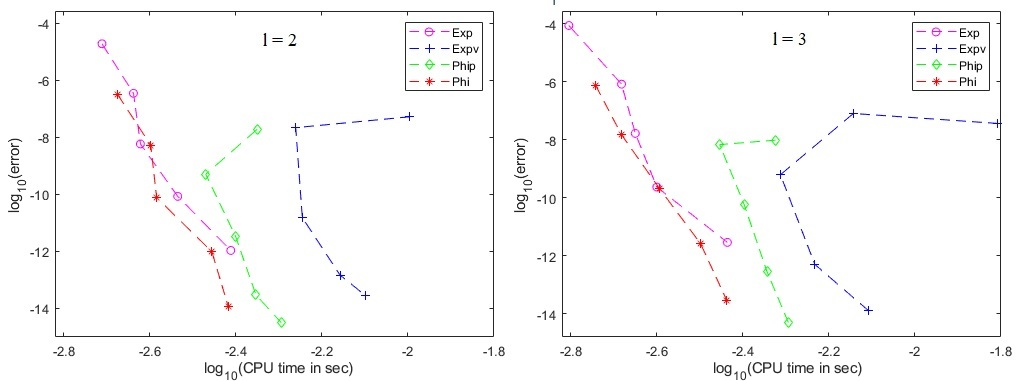
\includegraphics[scale=0.55]{Graphics/phil2l3.jpg}
	\caption{Diagrama tiempo-precisión para los métodos de \cite{hochbruck1997krylov}, \cite{sidje1998expokit}, \cite{niesen2012algorithm} y (\ref{phi_approx}), denotados por \textit{Exp}, \textit{Expv}, \textit{Phip} y \textit{Phi} respectivamente, como función de la dimensión de Krylov $\mf$, en el cálculo de  (\ref{sum2_phiXv}) para dos valores de $l$. Izquierda $l=2$, Derecha $l=3$. De arriba hacia debajo, $\mf=4,5,6,7,8$ para cada método, siendo $\mf=6$ el valor óptimo estimado como se especificó anteriormente con tolerancias $ATol=10^{-9}$ y $RTol=10^{-6}$.}
	\label{fig:SumPhi}
\end{figure}

\subsubsection{Simulaciones numéricas para Aproximaciones Krylov-Padé libre de Jacobiano}
Consideraremos el cálculo de (\ref{sum2_phiXv}) con matriz Jacobiana $f_x$ y campo vectorial $f$ del PVI resultante de discretizar una ecuación diferencial parcial. La siguiente matriz Jacobiana y la ecuación discretizada fue tomada de~\cite{tokman2006efficient}.

\begin{example}
	\label{ej:ej1-hpfj} Matriz Jacobiana de $2N\times2N$
	\begin{equation*}
	f_{x}(x)=\left[ 
	\begin{array}{cc}
	diag(2u\cdot v-4) & diag(u\cdot u) \\ 
	diag(3-2u\cdot v) & -diag(u\cdot u)%
	\end{array}%
	\right] +\frac{\alpha }{(\Delta z)^{2}}\left[ 
	\begin{array}{cc}
	K & 0 \\ 
	0 & K%
	\end{array}%
	\right] ,\text{ \ \ \ con \ \ \ \ }x=\left[ 
	\begin{array}{c}
	u \\ 
	v%
	\end{array}%
	\right] ,
	\end{equation*}
	\[
	K=\left[ 
	\begin{array}{ccccc}
	-2 & 1 &  &  & \\
	1 & -2 & 1 &  &  \\
	& \ddots  & \ddots  & \ddots  &  \\
	&  & 1 & -2 & 1 \\
	&  &  & 1 & -2%
	\end{array}%
	\right]_{N\times N}
	\]
	de la  ecuación $2N$-dimensional Brusselator discretizada
	\begin{eqnarray*}
		\frac{du_{i}}{dt} &=&1+u_{i}^{2}v_{i}-4u_{i}+\frac{\alpha }{(\Delta z)^{2}}%
		(u_{i-1}-2u_{i}+u_{i+1}) \\
		\frac{dv_{i}}{dt} &=&3u_{i}-u_{i}^{2}v_{i}+\frac{\alpha }{(\Delta z)^{2}}%
		(v_{i-1}-2v_{i}+v_{i+1})
	\end{eqnarray*}
	con $\alpha =1/50$, $u_{i}(0)=1+\sin (2\pi z_{i})$, $v_{i}(0)=3$, $z_{i}=i/(N+1)$, $\Delta z =1/(N+1)$, $i=1,\ldots,N$, y $N=800$.
\end{example}

Los códigos de Matlab \textit{JF1-Phi} y \textit{JF2-Phi} implementan la aproximación Krylov-Padé libre de Jacobiano (\ref{phi_approx_fj}) con $\beta=0$ y las diferencias finitas de primer y segundo orden respectivamente
\begin{equation}\label{finite-differences}
	g(x,u;\delta)=\frac{f(x+\delta u)-f(x)}{\delta}  \;\;\; \text{y} \;\;\; g(x,u;\delta)=\frac{f(x+\delta u)-f(x-\delta u)}{2\delta}
\end{equation}
donde $\delta= \frac{\sqrt{(1+||x||_2)\epsilon_{mach}}}{\epsilon_{mach}+||u||_2}$ como se sugiere en~\cite{knoll2004jacobian}, siendo $\epsilon_{mach}$ el épsilon de la máquina. El código de Matlab \textit{Phi} implementa la aproximación Krylov-Padé (\ref{phi_approx}) con la matriz exacta.

En el ejemplo, la matriz y los vectores en (\ref{sum2_phiXv}) se definen como $A=f_x(x(0))$, $a_1=a_2=f(x(0))$, $a_3=2a_1 $ y $a_4=6a_1$ de acuerdo con el número de términos $l$ en cada ejemplo. La norma euclidiana se usa para medir el error entre el valor ``exacto'' de $L e^{h M}r$ en (\ref{sum2_phiXv}) y sus aproximaciones. Para fines comparativos, el valor ``exacto'' de $e^{h M}$ y la matriz exponencial $\me{\tau\overline{H}}$ en los códigos \textit{JF1-Phi}, \textit{JF2-Phi} y \textit{Phi} se calculan con la misma función de Matlab \textit{expm}. La fila superior de la Figura \ref{fig:SumPhiBrusselator} presenta, para cada ejemplo, las gráficas logarítmicas de tolerancia relativa (\textit{rtol}) contra error (\textit{error}) en el cálculo de (\ref{sum2_phiXv}) mediante las aproximaciones \textit{JF1-Phi}, \textit{JF2-Phi} y \textit{Phi} con tolerancias relativas y absolutas $rtol=10^{-j}$ y $atol=0.1 rtol$, con $j=1,\ldots,6$. La fila inferior de esta figura presenta las gráficas de la dimensión de Krylov $\mf$ contra $log(rtol)$ correspondientes a las aproximaciones en la fila superior de las figuras. Los valores de $\mf$ son determinados automáticamente por cada código para cada una de las tolerancias especificadas $rtol$ y $atol$, tal y como se explicó anteriormente.

\begin{figure}[htb]
	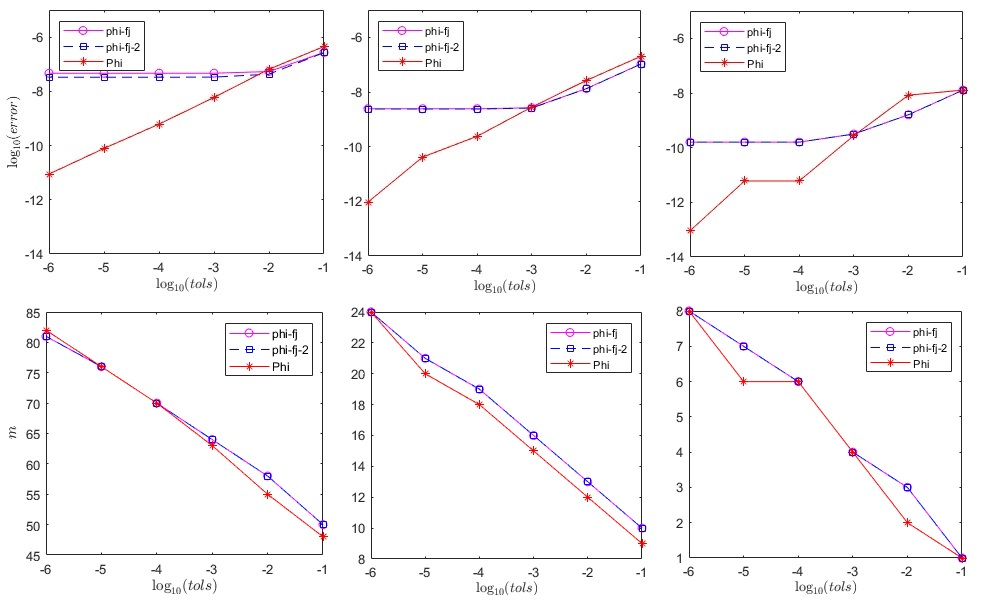
\includegraphics[scale=0.57]{Graphics/kpfj-brusselator-em.jpg}
	\caption{Superior: Gráficos Log-log de tolerancia relativa (\textit{rtol}) contra error (\textit{error}) en el cálculo de $\phi _{1}(f_x,h)a_{1}+\phi _{2}(f_x,h)a_{3}+\phi _{3}(f_x,h)a_{3}$ para la ecuación de ejemplo \ref{ej:ej1-hpfj} mediante las aproximaciones \textit{JF1-Phi}, \textit{JF2-Phi} y \textit{Phi} con $rtol=10^{-j}$ y $j=1,\ldots,6$. De izquierda a derecha, con $h=0.01,0.001,0.0001$. Inferior: Gráficos de tolerancia relativa (\textit{rtol}) contra dimensión de Krylov $\mf$ correspondiente a las aproximaciones de la figura superior.}
	\label{fig:SumPhiBrusselator}
\end{figure}

Observe que una diferencia importante entre las aproximaciones libre de Jacobiano y las de matriz exacta es el umbral para los errores de las primeras a medida que disminuye la tolerancia. Como es de esperar, cuando la tolerancia $rtol$ disminuye, la dimensión de Krylov $\mf$ para las tres aproximaciones aumenta y, en consecuencia, sus errores también disminuyen. Sin embargo, para valores crecientes de $\mf$, el valor fijo del segundo término de la derecha en (\ref{phi_approx_fj}) domina los valores decrecientes del primer término, lo que explica los umbrales para los errores de las aproximaciones libres de Jacobiano \textit{JF1-Phi} y \textit{JF2-Phi} en la Figura \ref{fig:SumPhiBrusselator}. Como se predice en (\ref{phi_approx}), el error de la aproximación con Jacobiano exacto \textit{Phi} en esta figura siempre disminuye cuando $\mf$ aumenta. Nótese también que, en correspondencia con el segundo término de la cota (\ref{phi_approx_fj}), la precisión de la aproximación con diferencia finita de segundo orden \textit{JF2-Phi} es ligeramente superior a la de la aproximación con diferencia finita de primer orden \textit{JF1-Phi} solo para los valores grandes de $h$ (gráfico superior izquierdo en la figura).

Las simulaciones numéricas corroboraron las principales implicaciones del análisis de errores para dicha aproximación libre de Jacobiano, es decir; el umbral para los errores disminuye cuando aumenta la dimensión del subespacio de Krylov; es menor el error de la aproximación con diferencia finita de segundo orden y  las aproximaciones libres de Jacobiano son menos precisas que las que utilizan matriz exacta.